\subsection{Examples of fANOVA decomposition}
% Known function, simulate input, plot fANOVA and PD, comparison

% PD and fANOVA: If inputs are independent, I think for the main effects fANOVA is simply PD shifted but fANOVA answers a different question than PD. PD usually asks for the effect of one specific variable on the prediction. In contrast, fANOVA decomposes the entire function. It is more about a global representation and clean, isolated effects because in sum they have to recover the original function and may not overlap.

\subsubsection*{Standard MVN, linear function, interaction}
Let us recall the fANOVA components from our first example of function $g(x_1, x_2) = x_1 + 2 x_2 + x_1 x_2$ under independence:
\begin{align*}
y_{\emptyset} &= 0, \\
y_1(x_1) &= x_1\\
y_2(x_2) &= 2x_2\\
y_{12}(x_1, x_2) &= x_1x_2.
\end{align*}
We can plot the main effects and the contour plot of the interaction term:
% Input: MVN, centred, independent
\begin{figure}[htpb]
    \centering
    \begin{minipage}[t]{0.49\textwidth}
        \centering
        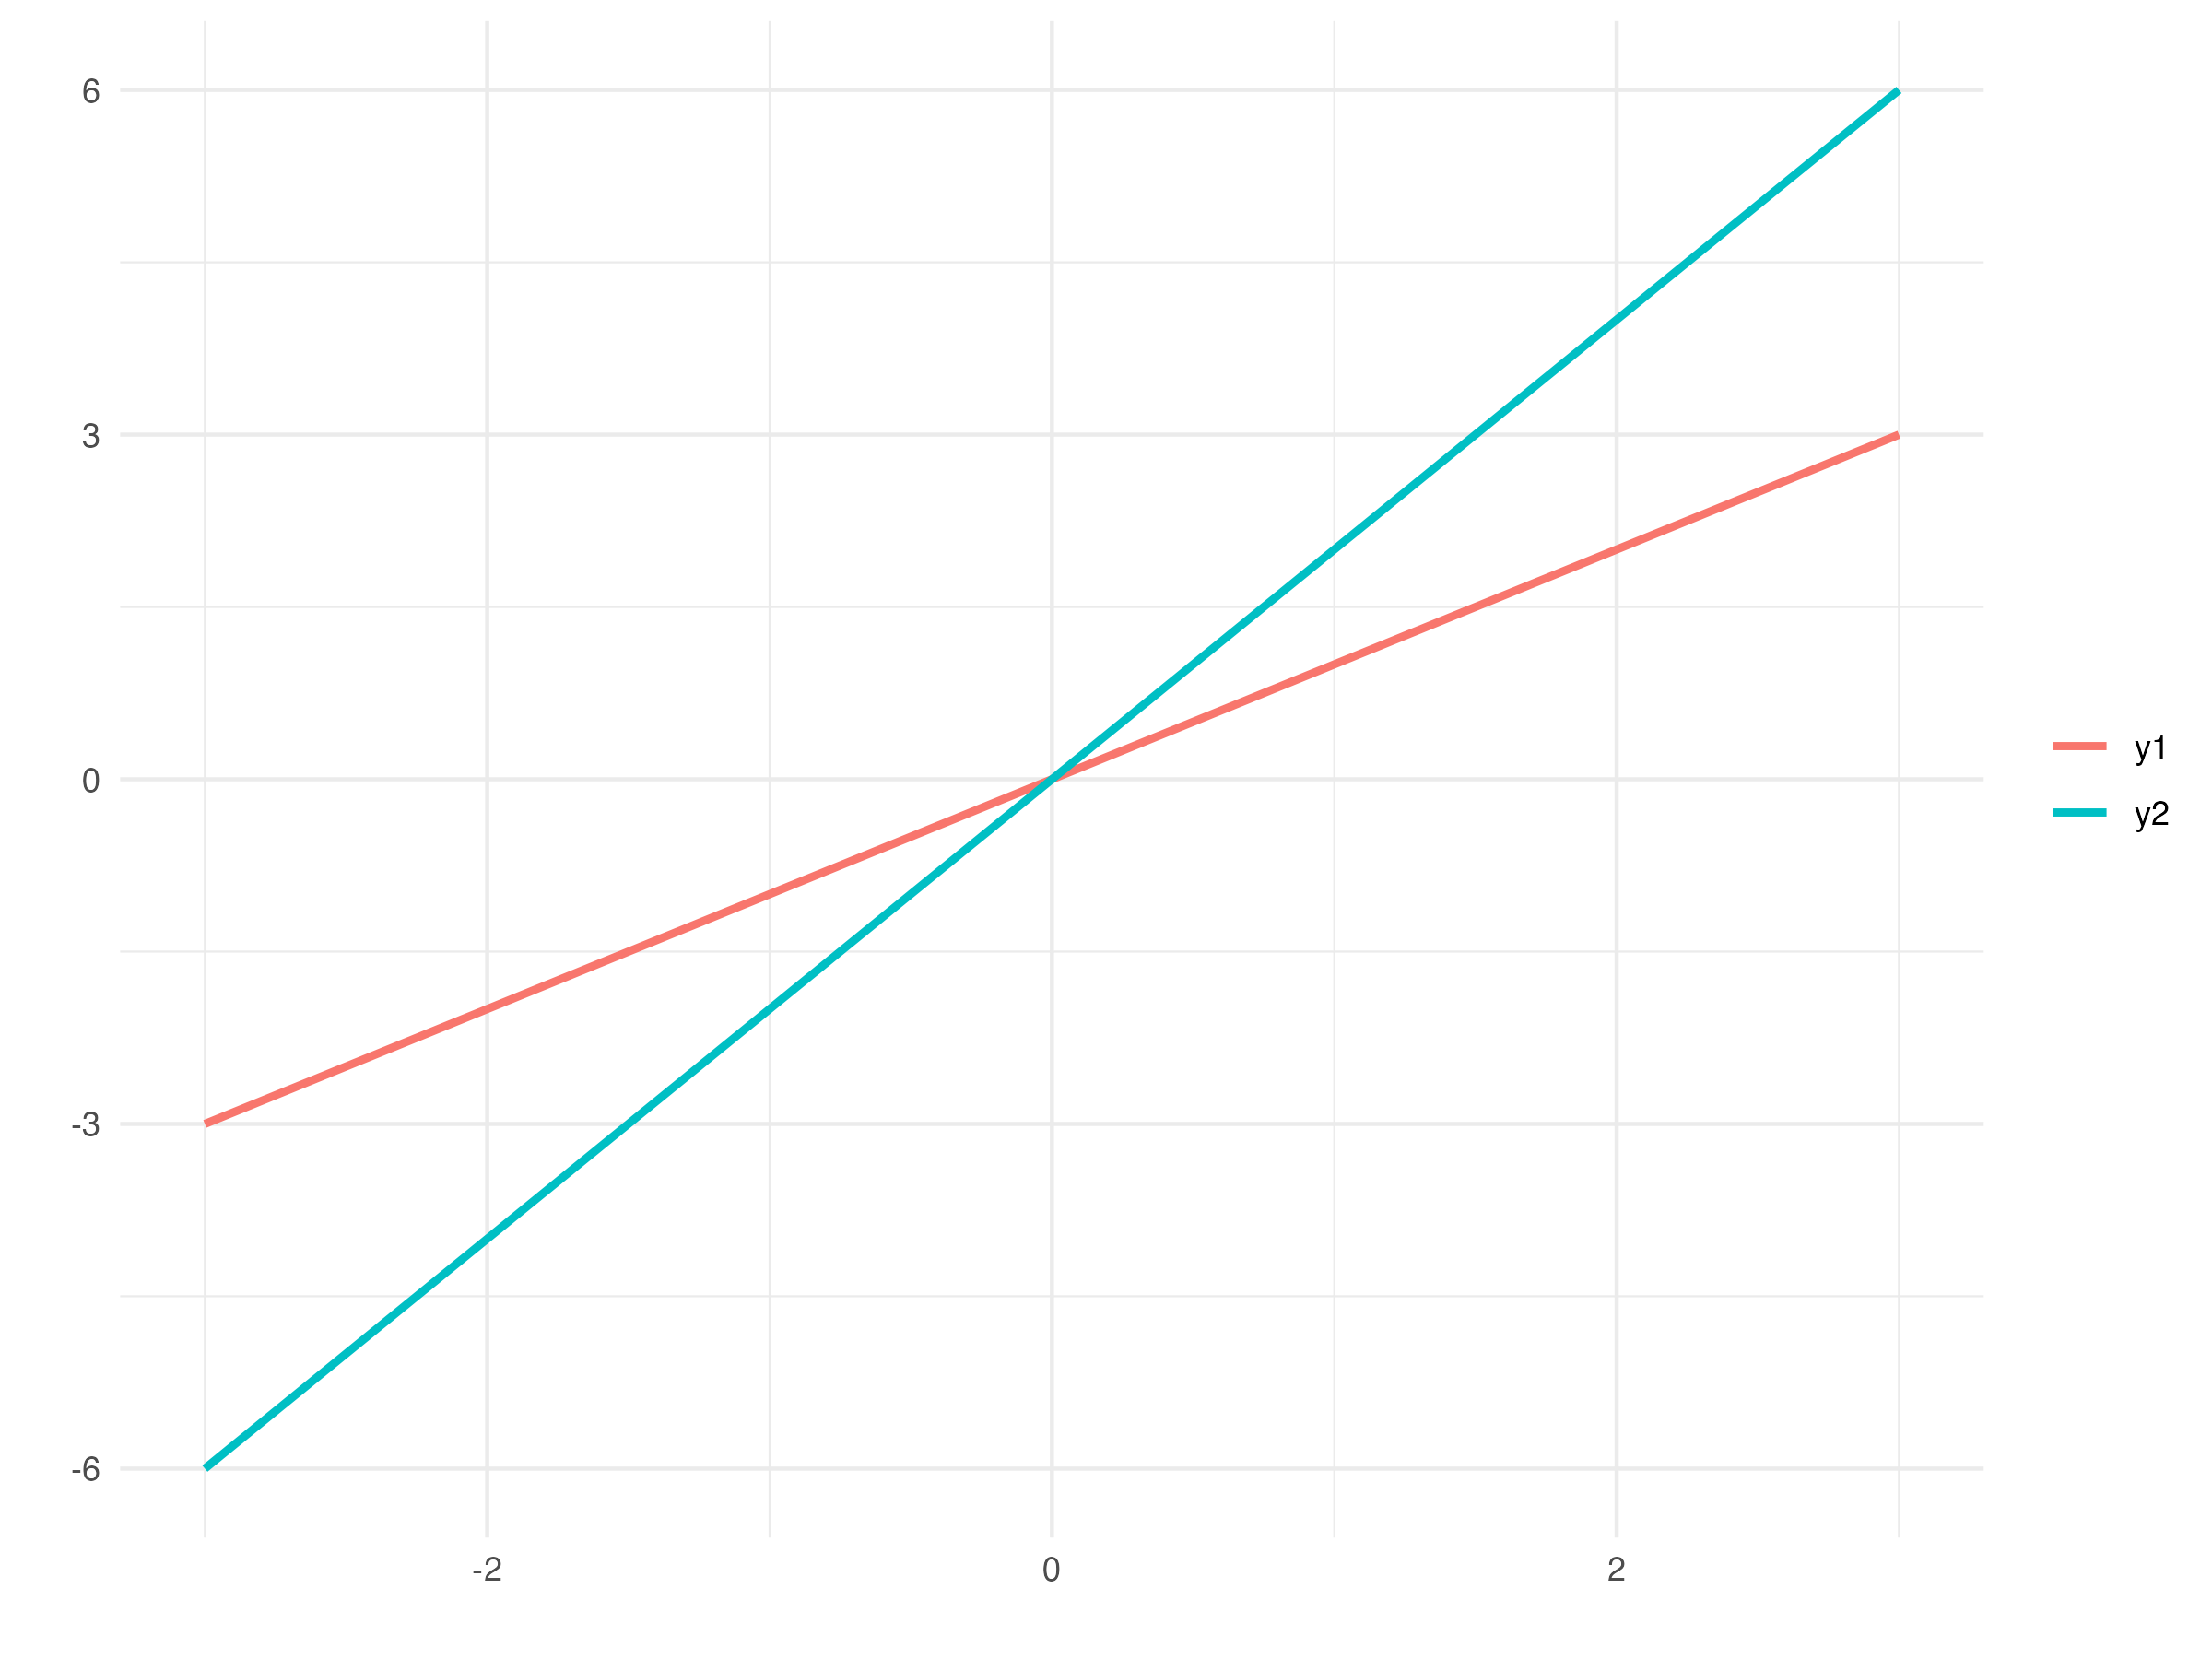
\includegraphics[width=\textwidth]{images/p_main_effect_ex1.png}
        \caption{Main terms as calculated via classical fANOVA for $g(x) = x_1 + 2 x_2 + x_1 x_2$.}
        \label{fig:main_effects_ex1}
    \end{minipage}%
    \hfill
    \begin{minipage}[t]{0.49\textwidth}
        \centering
        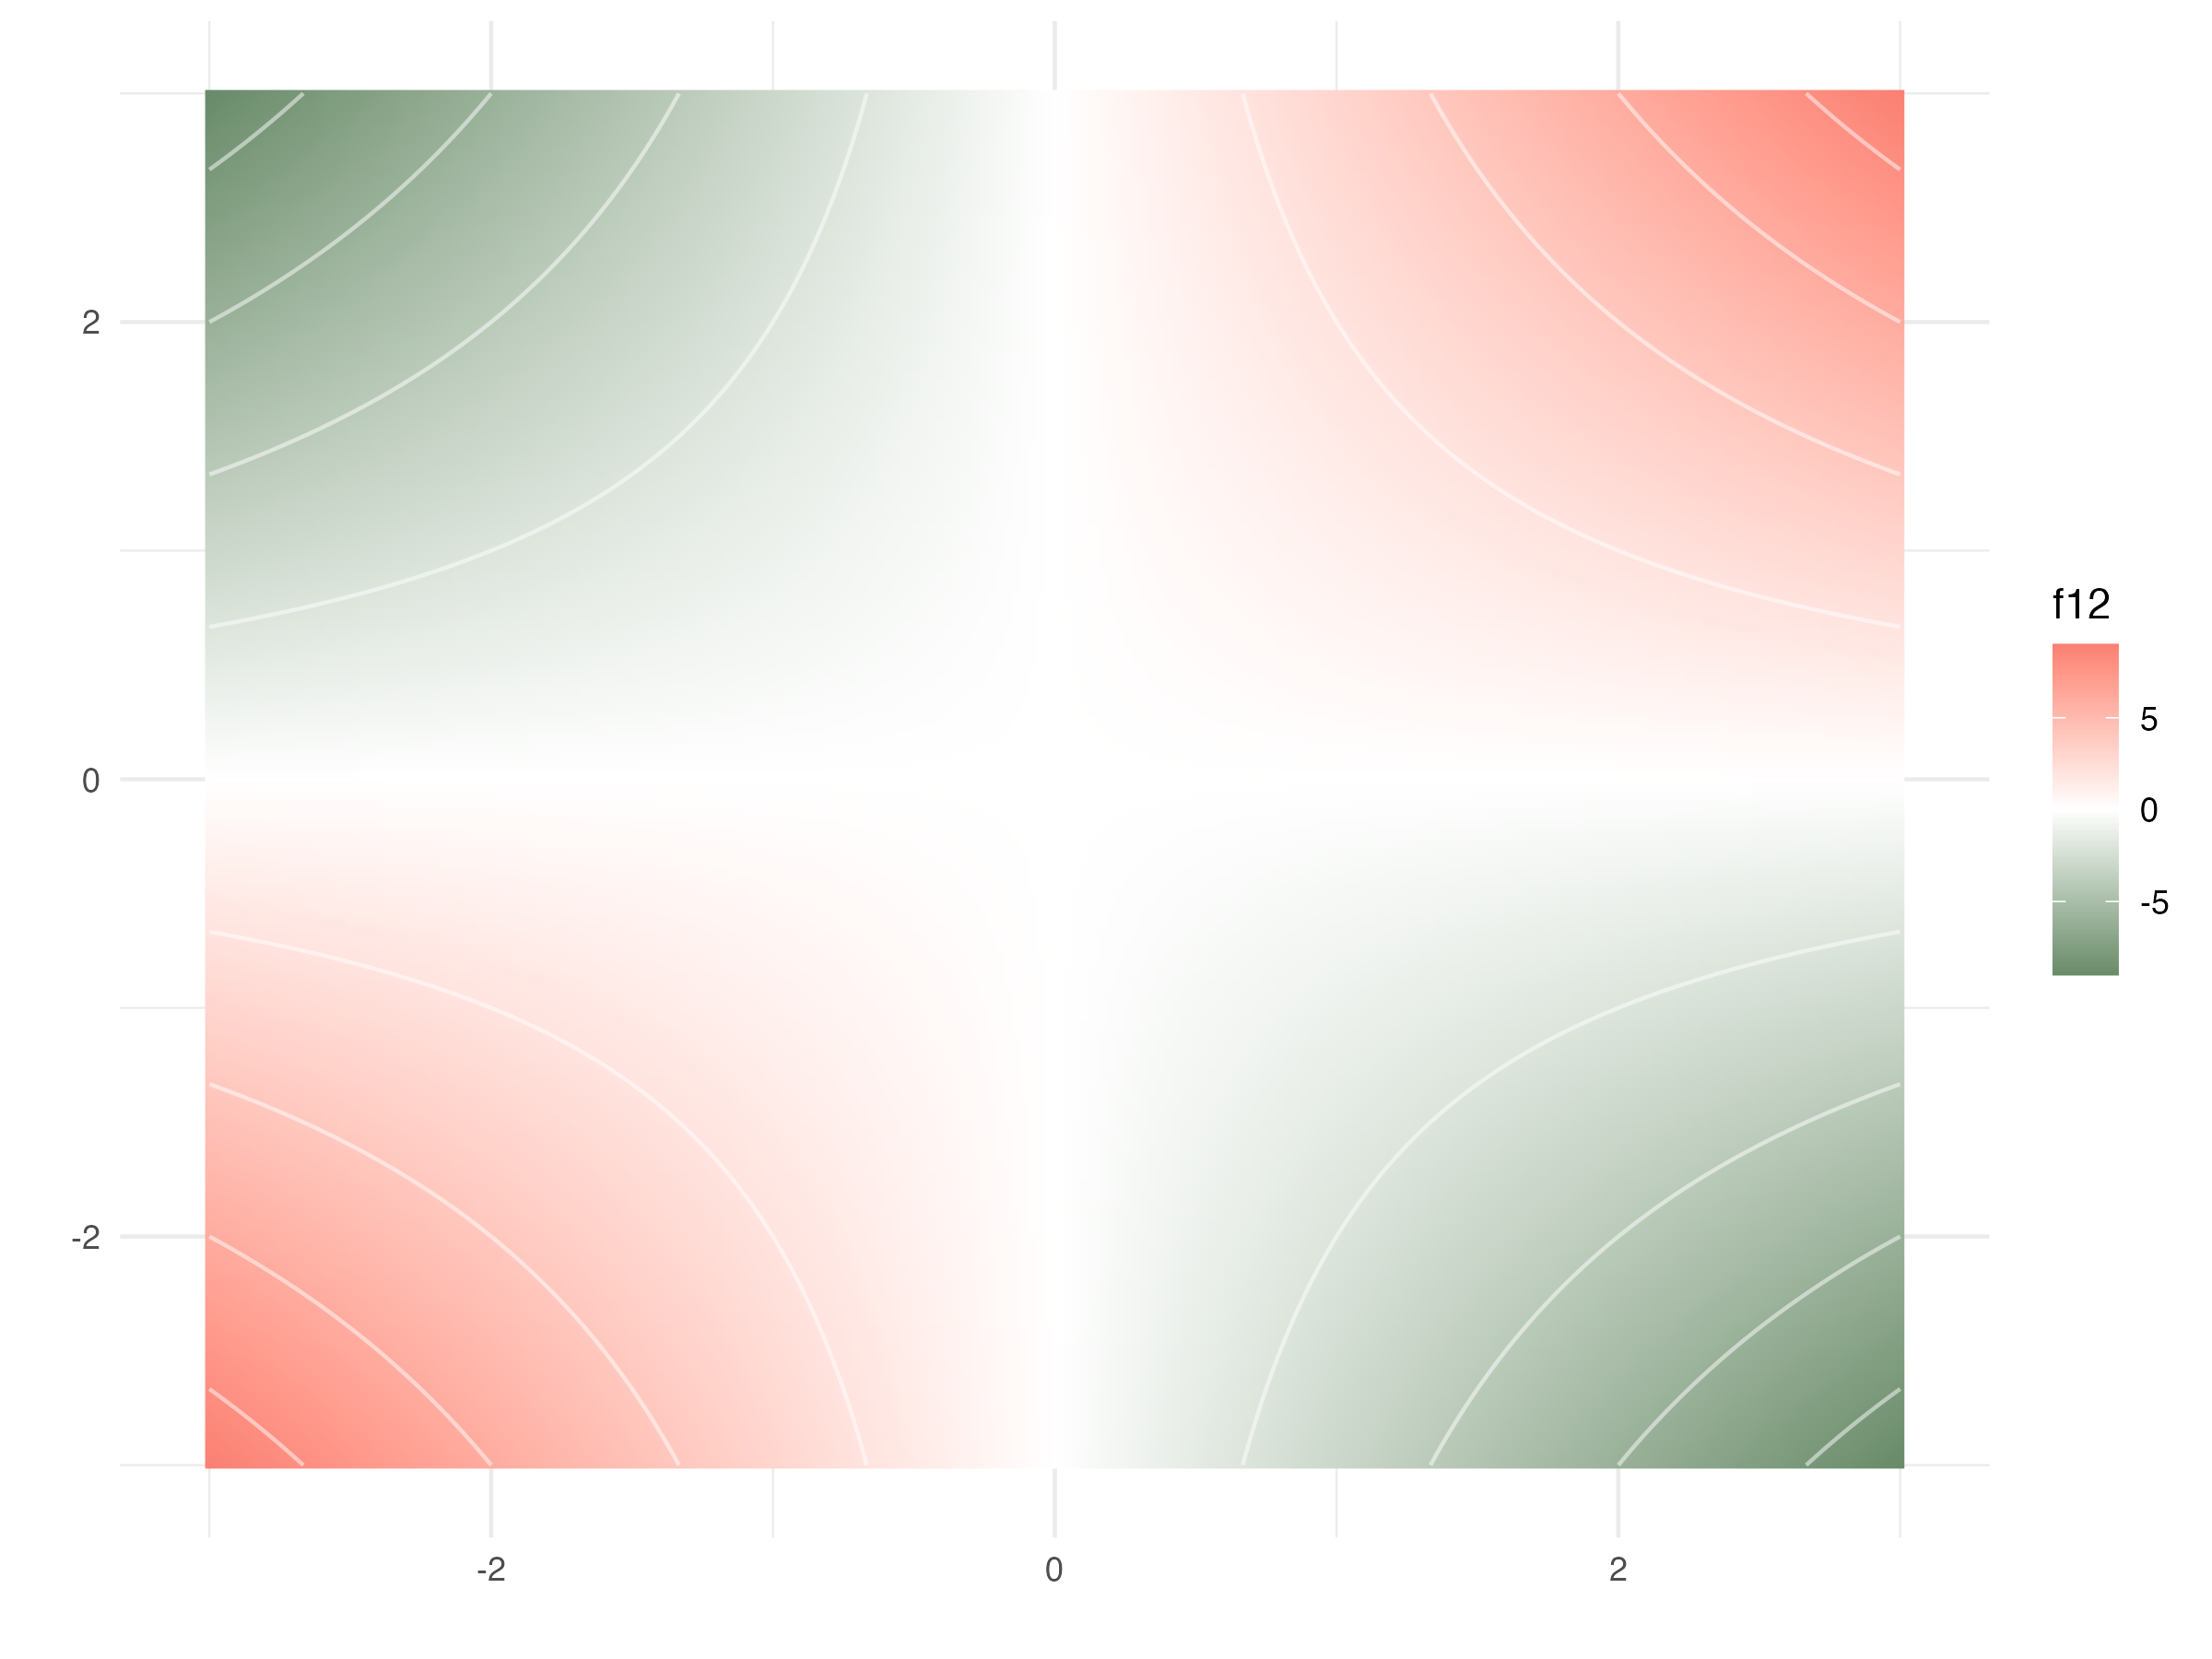
\includegraphics[width=\textwidth]{images/p_contour_ex1.png}
        \caption{Contour plot of $g(x) = x_1 + 2 x_2 + x_1 x_2$.}
        \label{fig:contour_ex1}
    \end{minipage}
\end{figure}

% \begin{figure}[htpb]
%     \centering
%     \begin{minipage}[t]{0.49\textwidth}
%         \centering
%         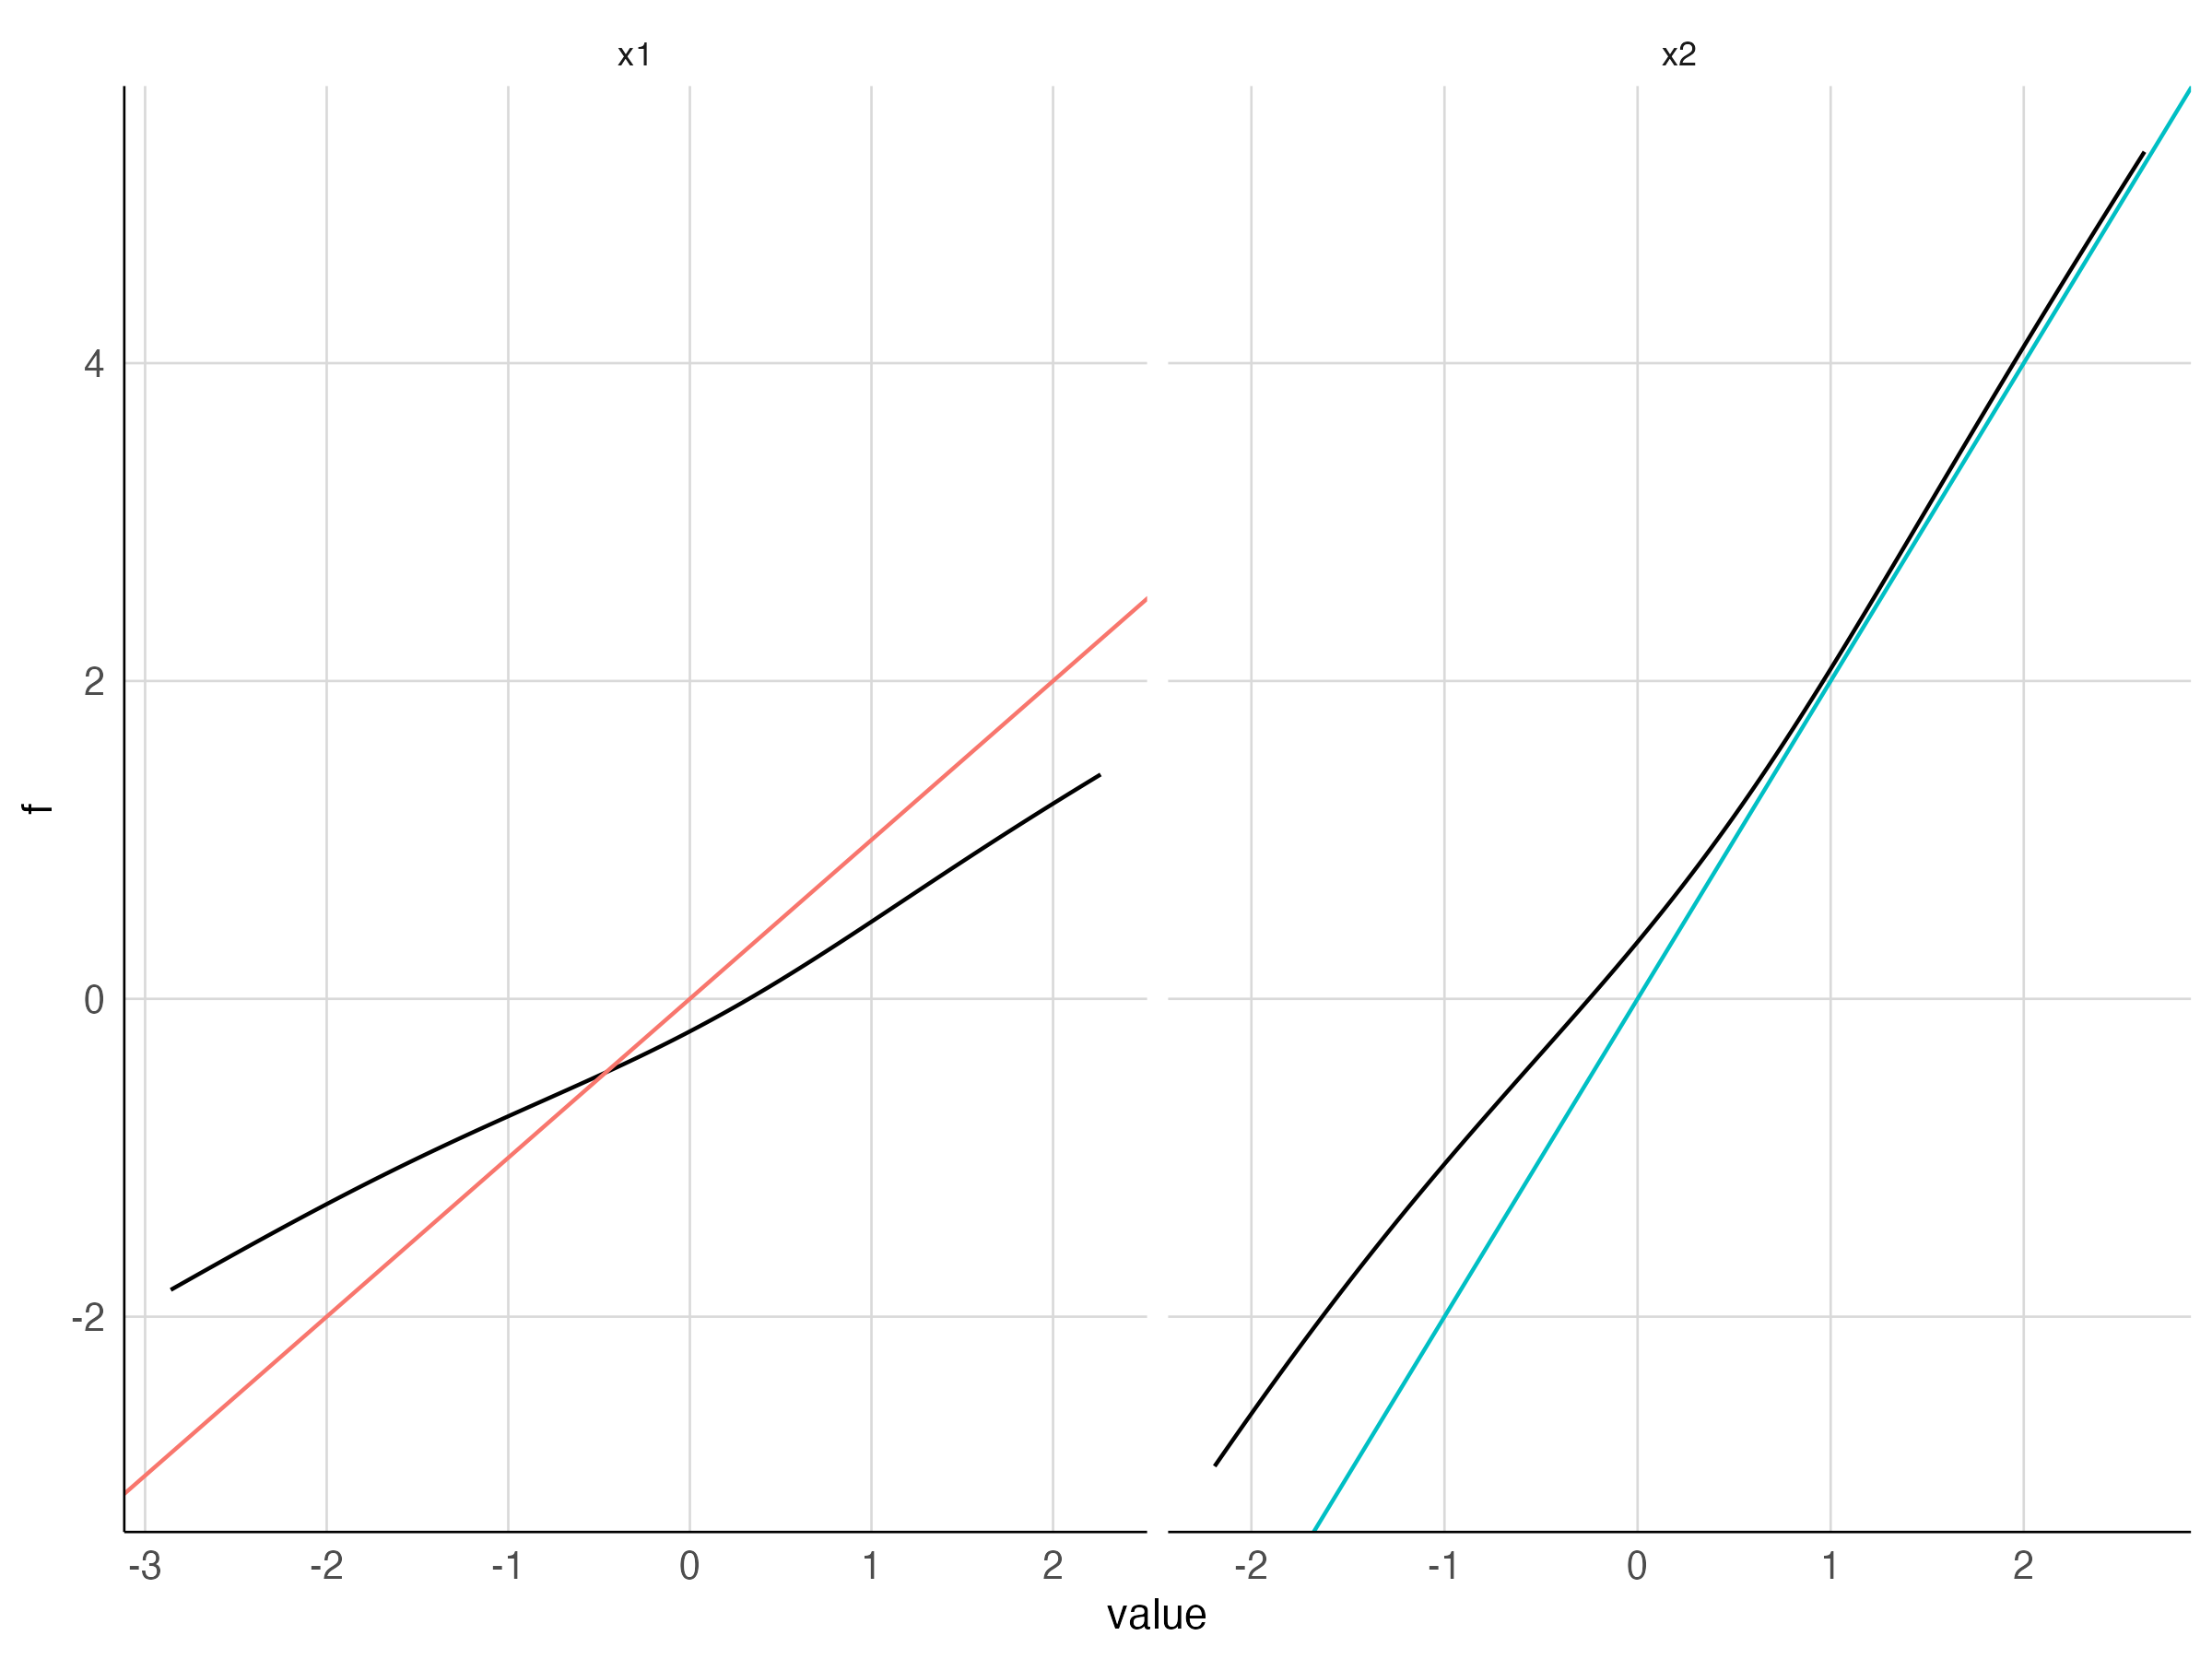
\includegraphics[width=\textwidth]{images/indep_150_main.png}
%         \caption{Estimation of Main terms as calculated via classical fANOVA for $g(x) = x_1 + 2 x_2 + x_1 x_2$ via Hooker method.}
%         \label{fig:indep_150_main}
%     \end{minipage}%
%     \hfill
%     \begin{minipage}[t]{0.49\textwidth}
%         \centering
%         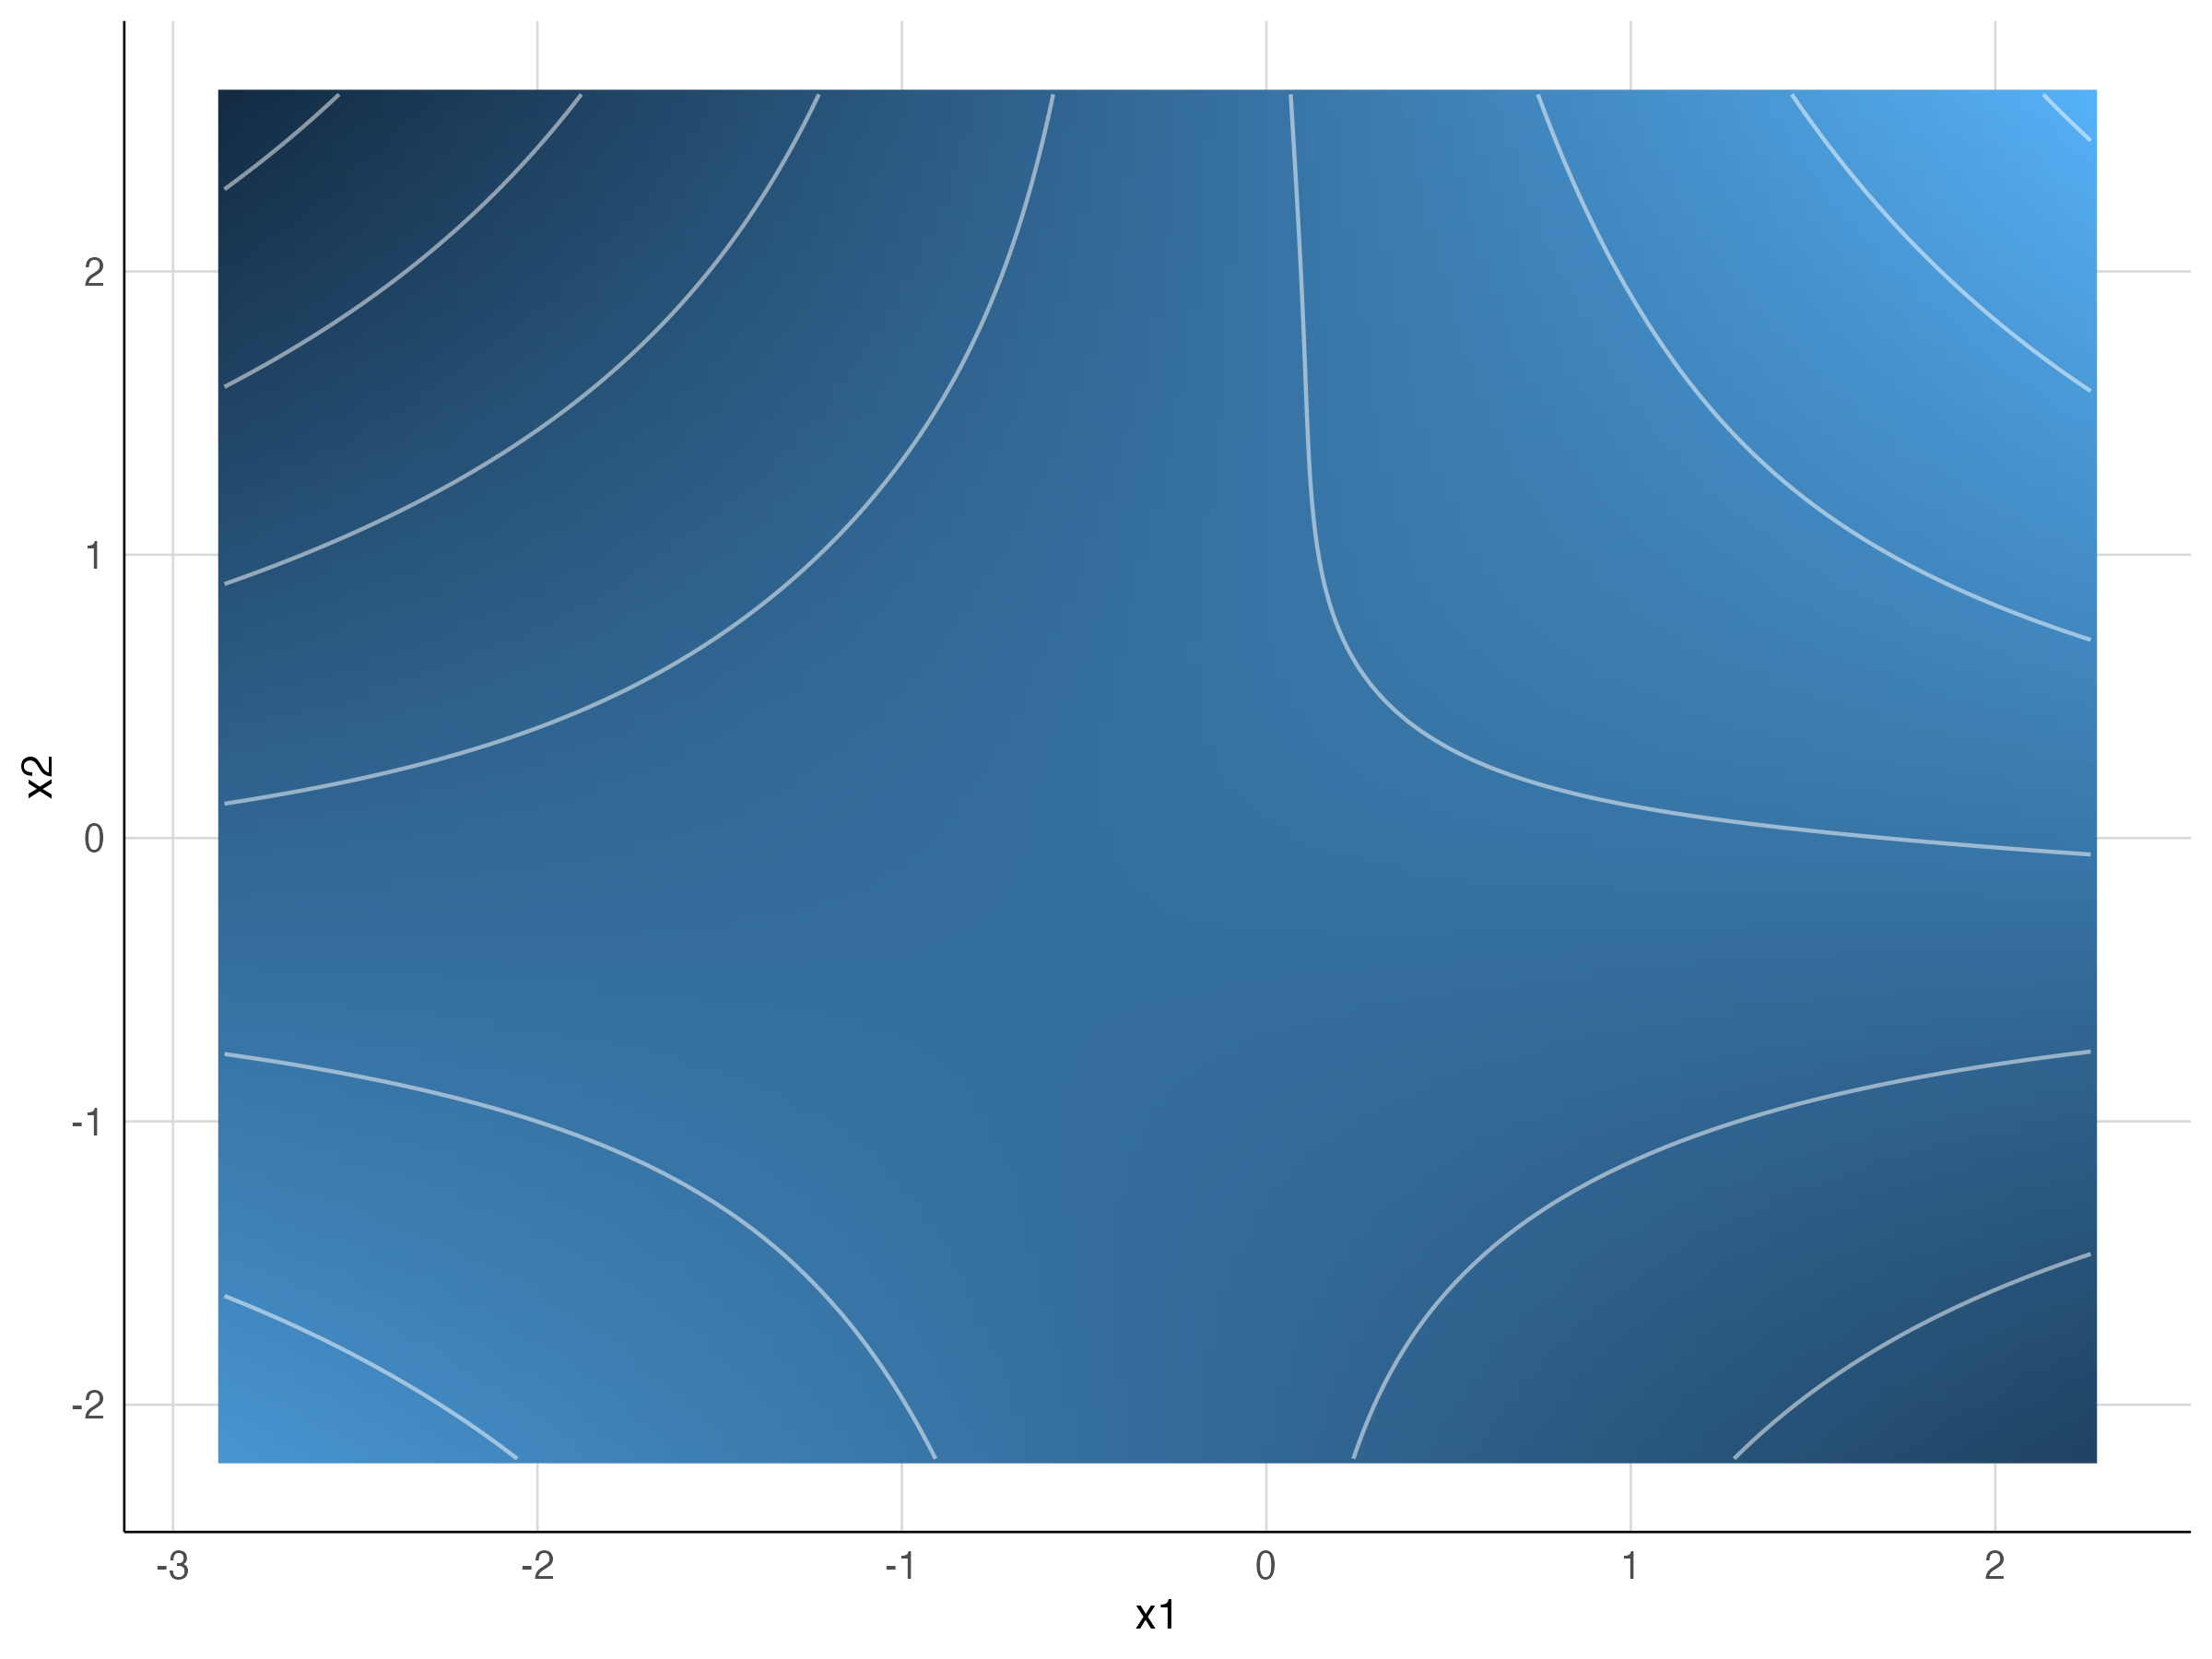
\includegraphics[width=\textwidth]{images/indep_150_interact.png}
%         \caption{Estimation of Contour plot of $g(x) = x_1 + 2 x_2 + x_1 x_2$ via Hooker method.}
%         \label{fig:indep_150_interact}
%     \end{minipage}
% \end{figure}

\subsubsection*{Standard MVN, linear function, interaction, dependent inputs}
% Zwei Plots für rho = 0.6 nebeneinander, jeweils halbe Breite
\begin{figure}[htpb]
    \centering
    \begin{minipage}[t]{0.49\textwidth}
        \centering
        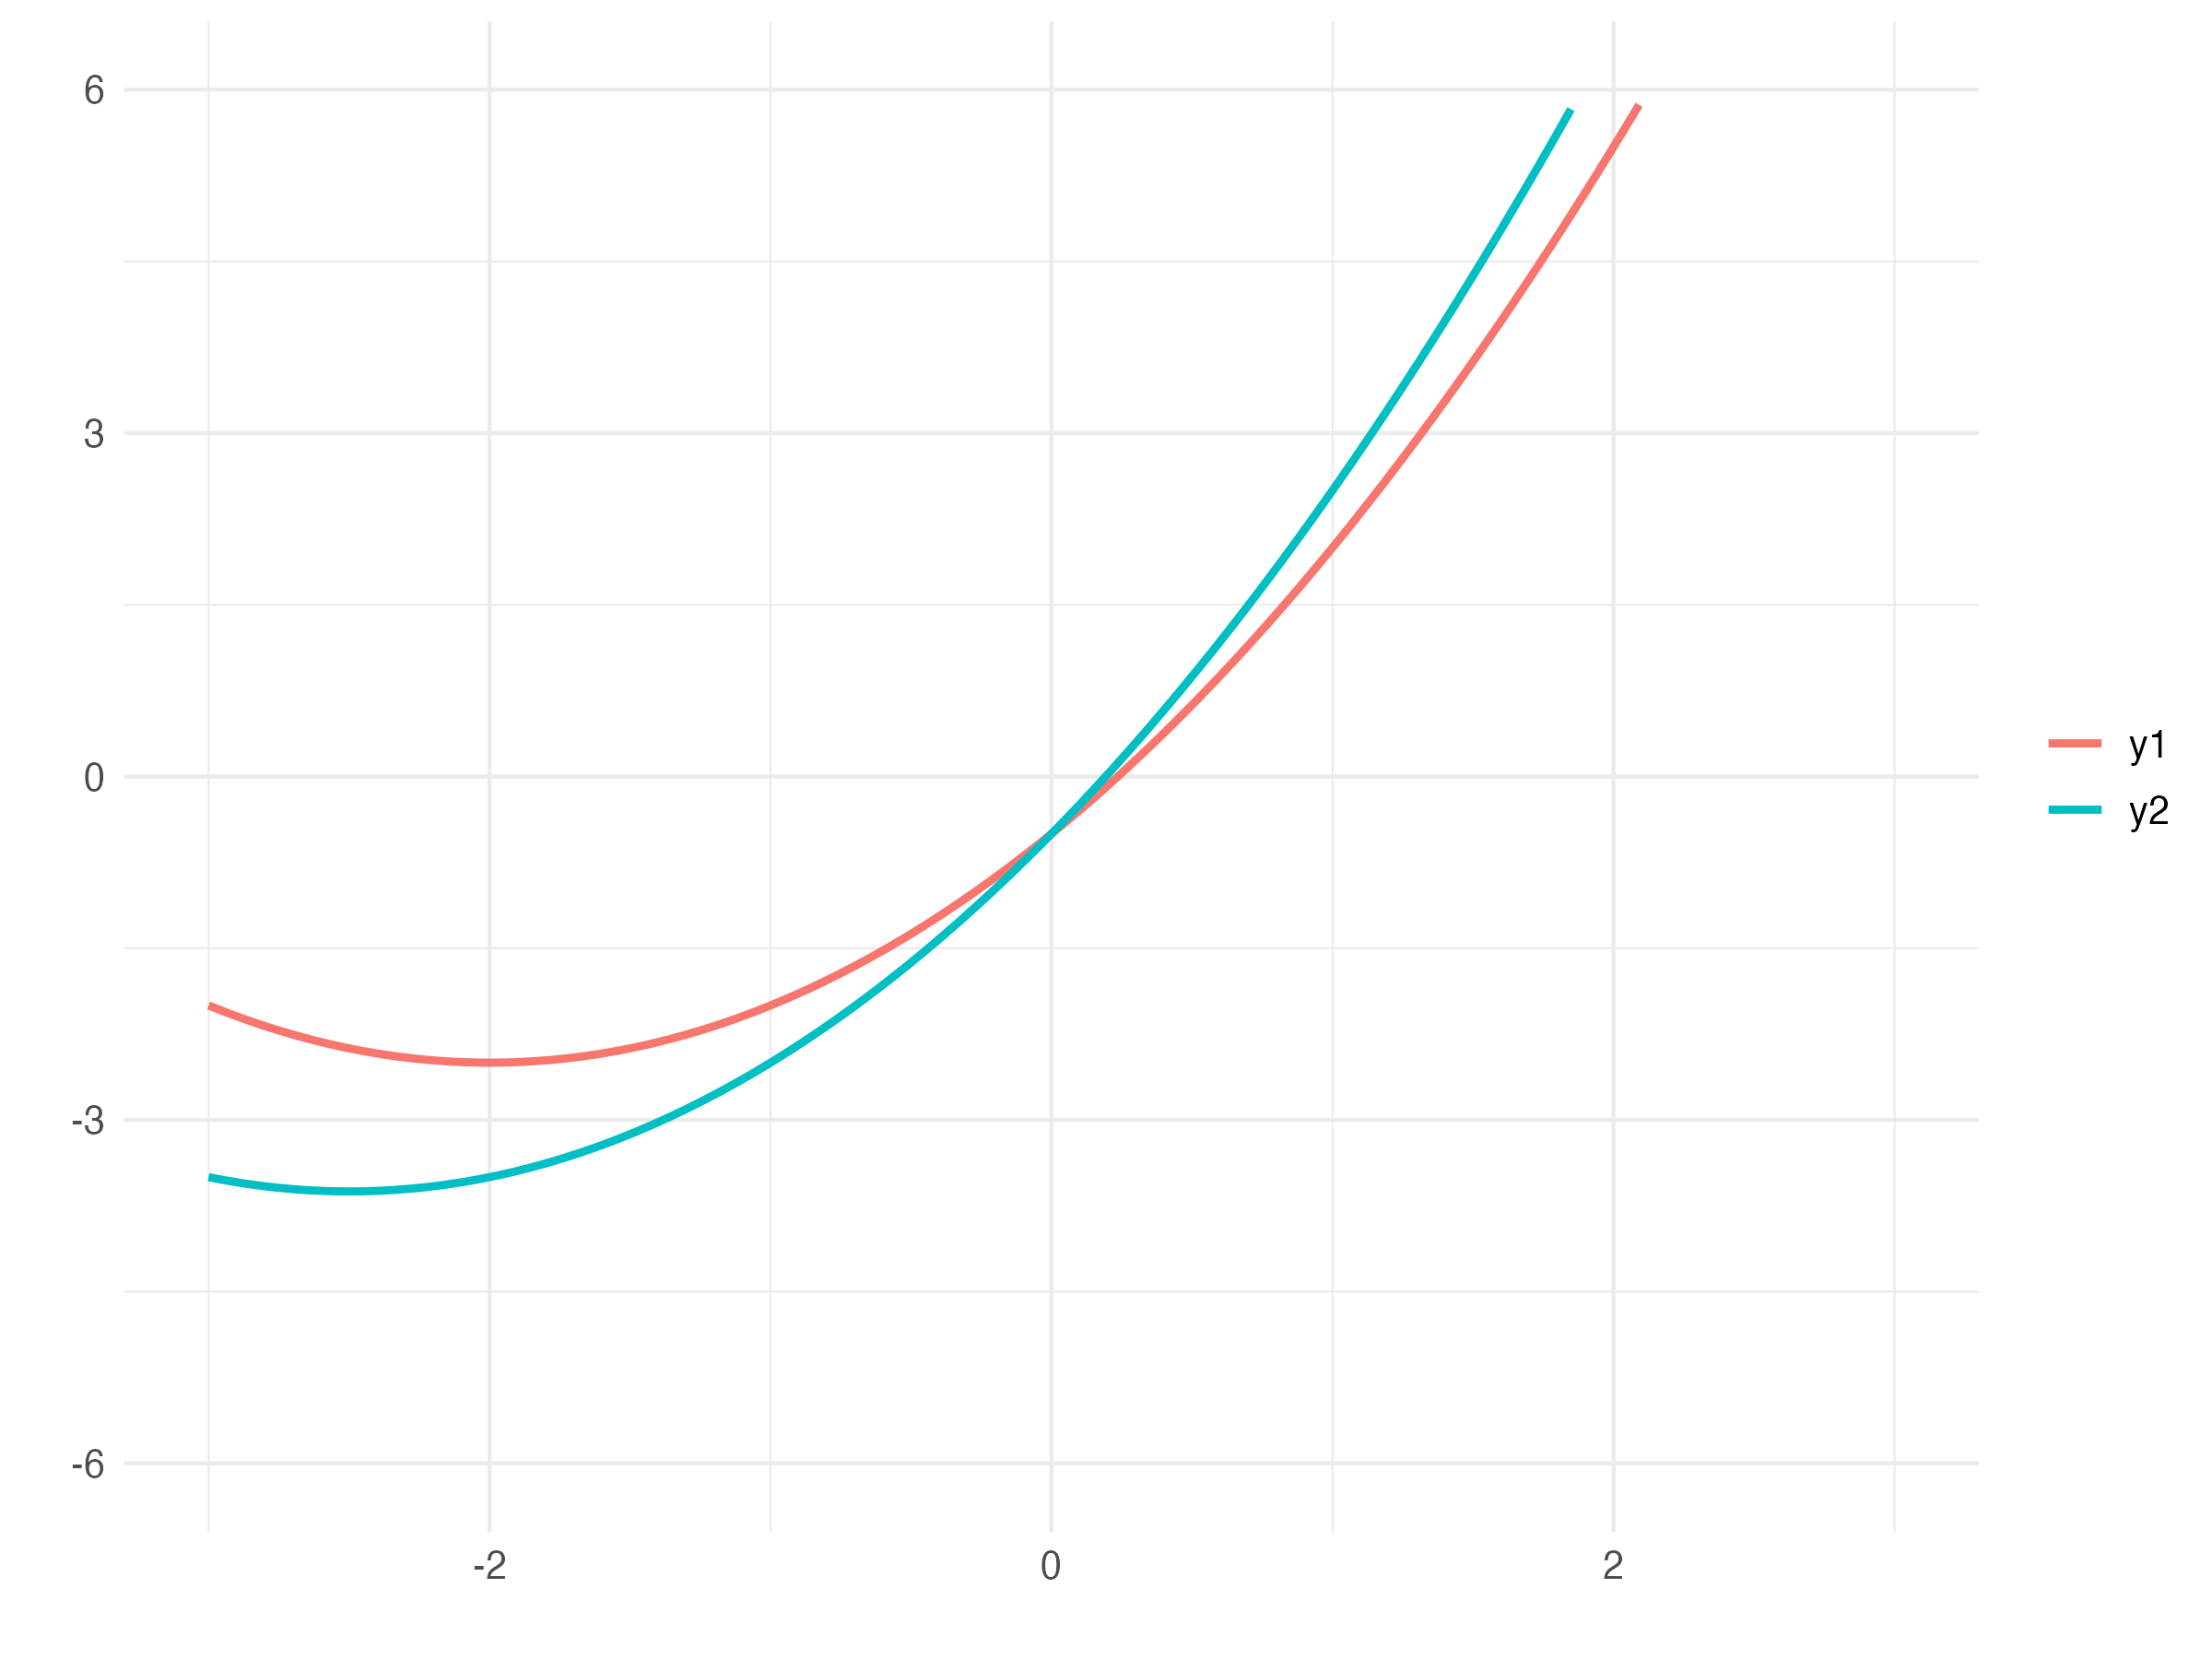
\includegraphics[width=\textwidth]{images/hoeffding_rho05.png}
        \caption{Hoeffding decomposition of $g(x) = x_1 + 2 x_2 + x_1 x_2$ with $\rho = 0.5$.}
        \label{fig:hoeffding_rho05}
    \end{minipage}%
    \hfill
    \begin{minipage}[t]{0.49\textwidth}
        \centering
        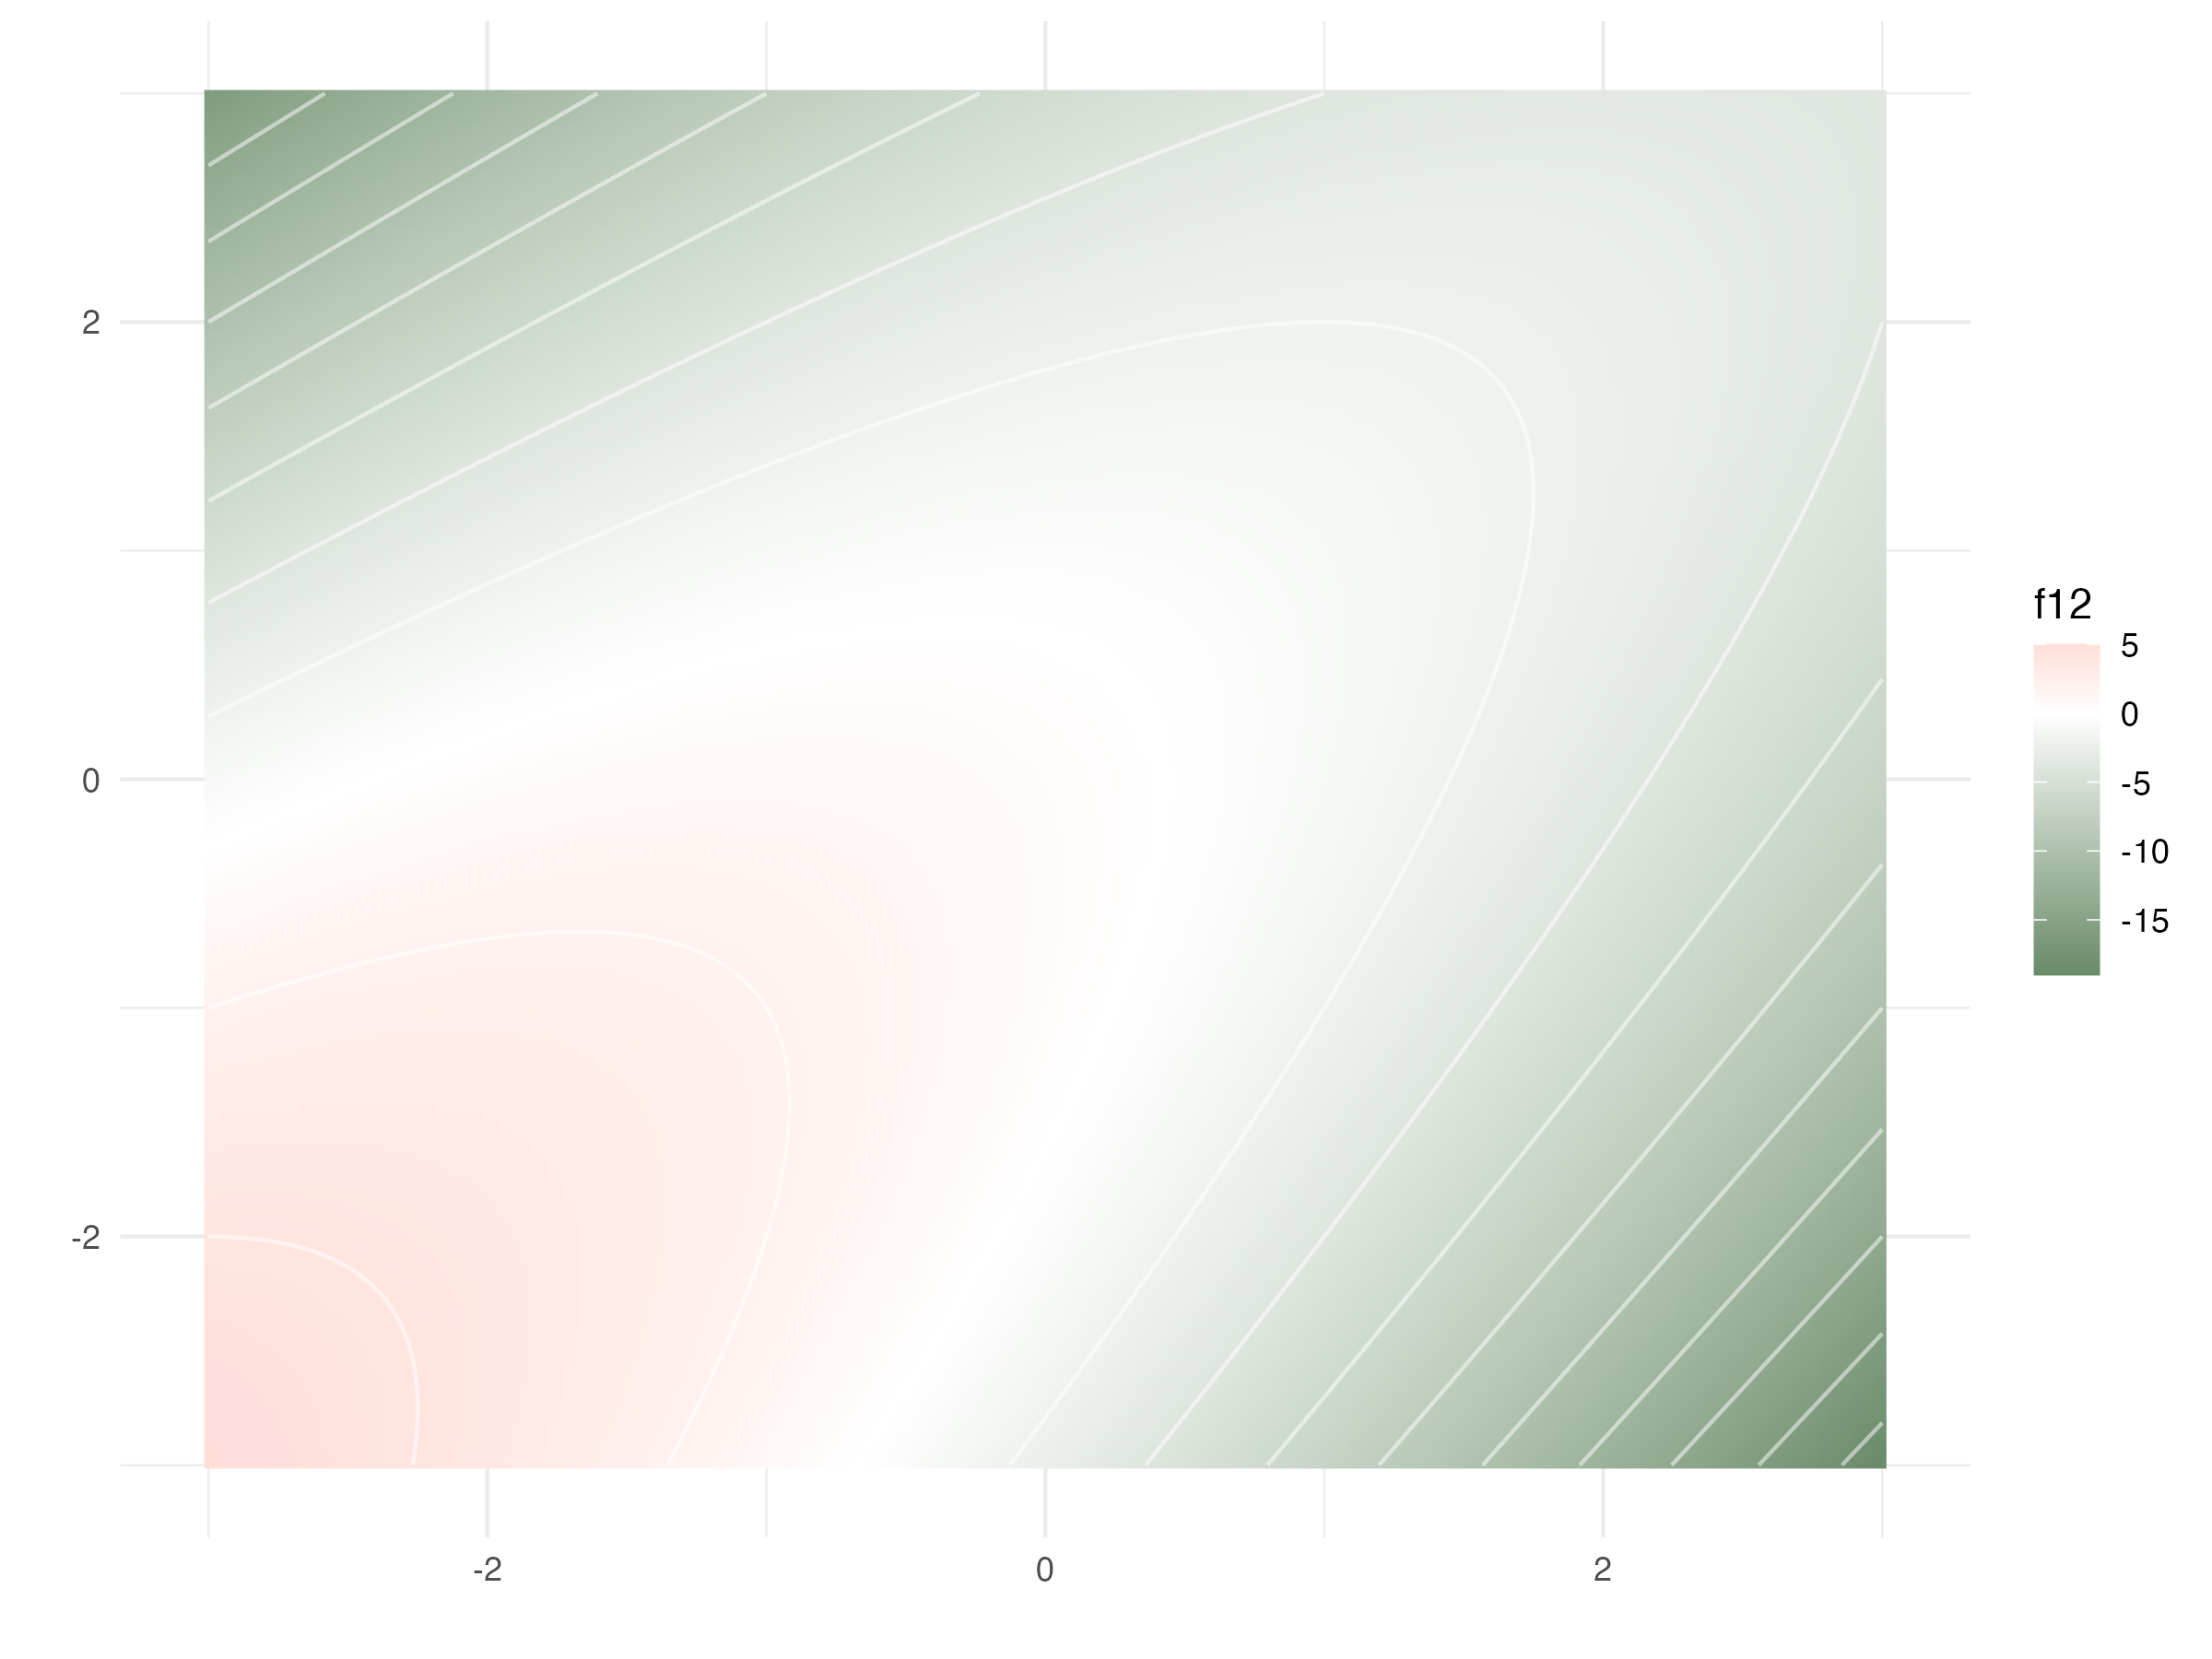
\includegraphics[width=\textwidth]{images/hoeffding_contour_rho05.png}
        \caption{Contour plot of $g(x) = x_1 + 2 x_2 + x_1 x_2$ with $\rho = 0.5$.}
        \label{fig:hoeffding_contour_rho05}
    \end{minipage}
\end{figure}

\subsubsection*{Estimated generalized fANOVA components}
\begin{figure}[htpb]
    % insert g1_1 and g1_2 as minipages
    \centering
    \begin{minipage}[t]{0.49\textwidth}
        \centering
        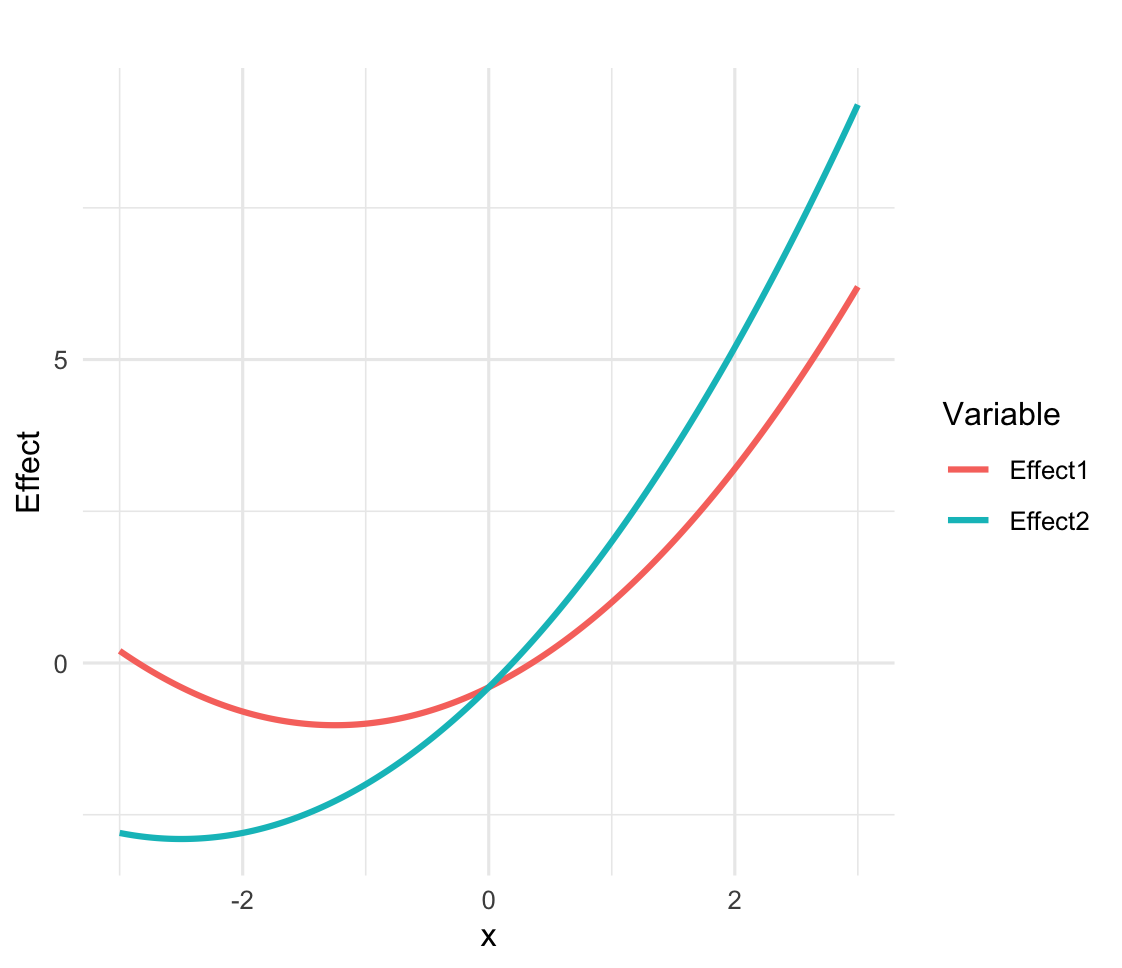
\includegraphics[width=\textwidth]{images/gpt_func_main.png}
        \caption{Generalized main effects for $g(x) = x_1 + 2 x_2 + x_1 x_2$ with dependent inputs, $\rho = 0.5$.}
        \label{fig:dep_150_main}
    \end{minipage}%
    \hfill
    \begin{minipage}[t]{0.49\textwidth}
        \centering
        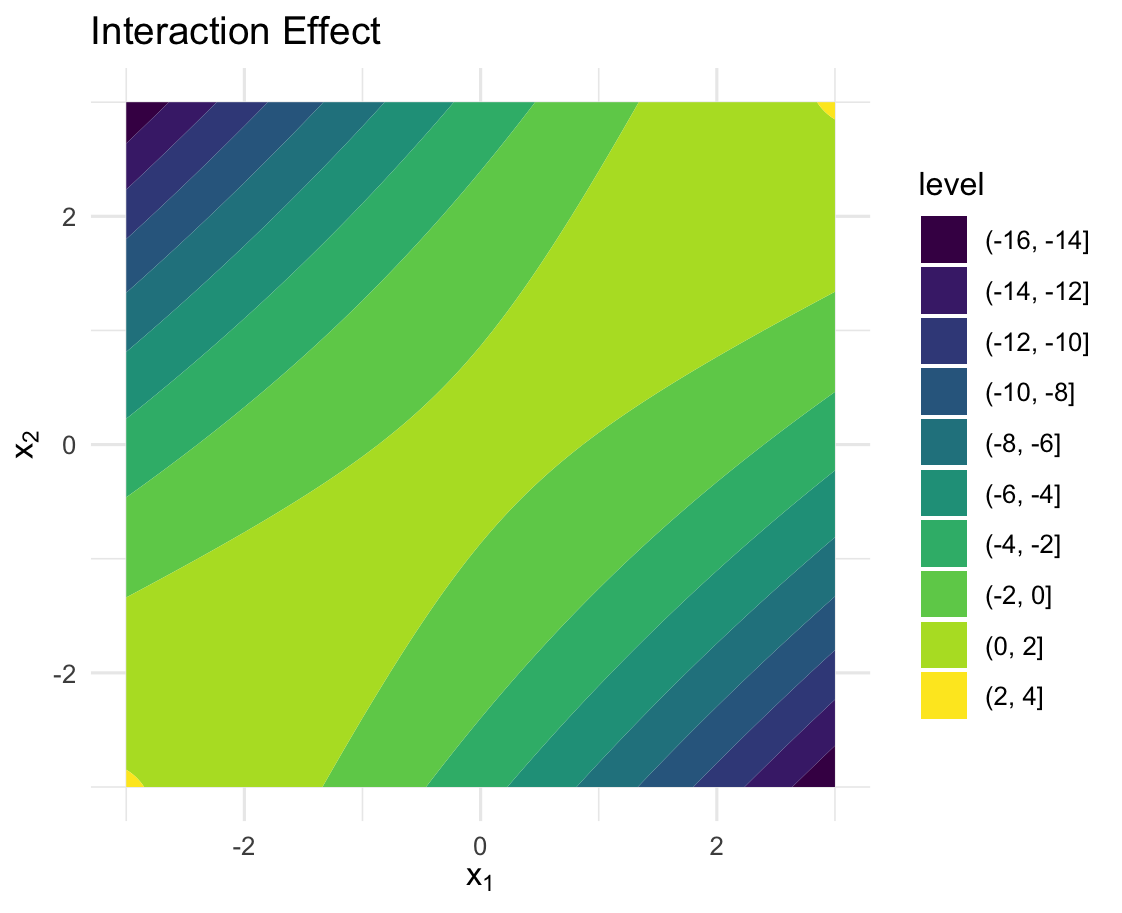
\includegraphics[width=\textwidth]{images/gpt_func_interaction.png}
        \caption{Contour plot of generalized interaction term for $g(x) = x_1 + 2 x_2 + x_1 x_2$ with dependent inputs, $\rho = 0.5$.}
        \label{fig:dep_150_interact}
    \end{minipage}
\end{figure}

